\documentclass[a4paper]{jarticle}
\usepackage{tani_resume}
\usepackage{epstopdf}
\usepackage{graphicx}
\usepackage{ascmac}
\alignbeforeskip -5mm
\alignafterskip -5mm
\eqnarraybeforeskip -5mm
\eqnarrayafterskip -5mm

\makeatletter
\newenvironment{figurehere}
  {\def\@captype{figure}}
  {}
\makeatother

\jptitle{ビーバーコンテストタイトル\\フランスのソース}
\etitle{}
\jpauthor{鈴木一至 佐々木陽広}
\eauthor{Kazushi Suzuki,Akihiro Sasaki}
\course{谷聖一研究室}
\year{27}


%% 概要 %%
\abstract{

コンピュータ・サイエンスの普及を目的とした取り組みは,様々なところで行われている.
その中の1つに,小・中・高校生を対象にした「ビーバーコンテスト」がある.本演習では、オープンソースとして公開されているフランスのビーバーコンテストのソースコードを元に、実際のビーバーコンテストと同様にコンテストを受けれる環境の実装を実現した。}
%\compheading

\begin{document}
\maketitle
\begin{multicols}{2}
\setcounter{page}{27}

\section{はじめに}

\subsection{ビーバーコンテストとは}
(未編集)\\
ビーバーコンテスト(\cite{bebras-contest, bebras-pdf})とは,情報科学の基礎と情報通信技術活用に関する国際コンテストであり,対象学年は日本の小学校5年生から高等学校3年生までとなっている.2004年にリトアニアで始められ,2013年には世界29カ国 728,328人の児童・生徒が参加している.日本は2011年度から正式参加している.コンピュータ・サイエンスの事前知識がなくても解くことが可能な問題を扱い,問題を解くことによってコンピュータ・サイエンスの概念に触れることができ,論理的思考を向上させる一助になるようなものなっている.また,コンテスト形式ではあるが参加者に優劣をつける目的ではなく情報学の普及を目的とした活動である.

\subsection{目的}
現在、ビーバーコンテストを受けるには遠くのオランダのサーバーに接続する必要があり、コンテストを受ける環境によっては上手く問題を受けることができない場合があった。これを解消するために、手元の環境で実装し、主に日本からコンテストを受ける際に正常に動作できるようにすることが本演習の目的である。

\subsection{演習内容}
ブラウザ等で実際にコンテストを受けることができるコンテンツを作成した。\\
画像表示テスト\\
\begin{figurehere}
\begin{center}
	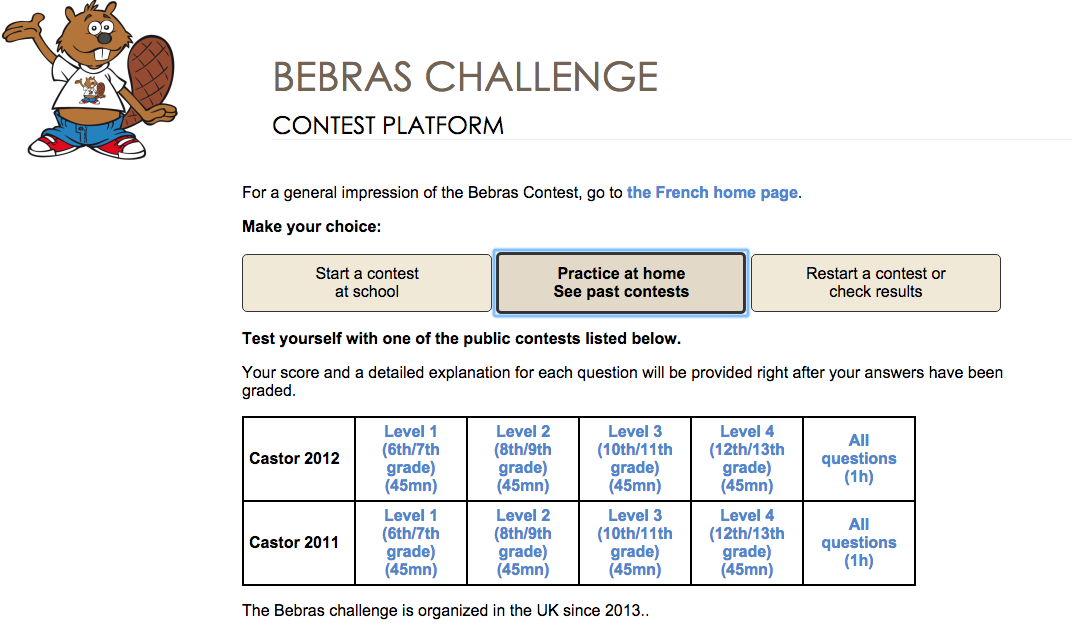
\includegraphics[bb=400 0 650 633,scale= 0.25]{img/bebras-test-form.png}\\
\end{center}
	\caption{スクリーンショット}\label{fig:1}
\end{figurehere}

(以下未編集)\\

\section{準備}

\begin{description}
\item[HTML5]  
\end{description}

\section{試行錯誤による理解促進}
非対話型問題のうち,4題が,試行錯誤させることで児童・生徒の理解促進がはかれると考え,試行錯誤可能なコンテンツを試作した.以下で試作したコンテンツを説明する.

\subsection{みつばちロボット}
\begin{itembox}[l]{問題}
ビ太郎はみつばちのロボットを作りました。\\このロボットは床に線を描いたり、線の上を飛ぶことができます。
\begin{itemize}
\item[四角]\mbox{}\\  \includegraphics[bb=0 0 160 60,width=3cm]{img/bee_rect.png}
\item[三角]\mbox{}\\  \includegraphics[bb=0 0 146 48,width=3cm]{img/bee_triangle.png}
\item[進む]\mbox{}\\  \includegraphics[bb=0 0 192 72,width=3cm]{img/bee_go.png}
\item[回る]\mbox{}\\  \includegraphics[bb=0 0 303 64,width=4cm]{img/bee_turn.png}
\end{itemize}
「四角,進む,回る,進む,三角」の命令を受け取ると,みつばちはこのような図形を描きます。
\begin{center}
\includegraphics[bb=0 0 568 88,width=7cm]{img/bee_example.png}
\end{center}
どのような命令を受け取ると、みつばちは次の絵を描くでしょうか?
\begin{center}
\includegraphics[bb=0 0 96 90,width=1cm]{img/bee_problem.png}
\end{center}
\begin{center}
\begin{tabular}{|p{5cm}|} \hline
四角,回る,進む,三角\\ \hline
四角,進む,回る,三角\\ \hline
三角,回る,四角\\ \hline
四角,進む,四角,回る,三角\\ \hline
\end{tabular}
\end{center}
{ \scriptsize 引用元:みつばちロボット. 「ビーバーコンテスト」情報ページ. http://bebras.eplang.jp/index.php?2014-みつばちロボット, (参照 2014-01-28)}
\end{itembox}

解説Webページでは静止画の連続での説明のみで,実際の処理を確認することができない.そこで,命令を与えると実際に動作する動的コンテンツを作成することで,児童・生徒が試行錯誤しながら考える事ができるようにした(図\ref{fig:1}〜図\ref{fig:4}参照).
\begin{figurehere}
\begin{center}
	\includegraphics[bb=0 0 620 554,width=6cm]{img/3_1_1.png}\\
\end{center}
	\caption{スクリーンショット (従来の教員向け解説)}\label{fig:1}
\end{figurehere}
\begin{figurehere}
\begin{center}
	\includegraphics[bb=0 0 620 591,width=6cm]{img/3_1_2.png}\\
\end{center}
	\caption{スクリーンショット (児童・生徒向け動的コンテンツ1)}\label{fig:2}
\end{figurehere}
\begin{figurehere}
\begin{center}
	\includegraphics[bb=0 0 620 606,width=6cm]{img/3_1_3.png}\\
\end{center}	
	\caption{スクリーンショット (児童・生徒向け動的コンテンツ2)}\label{fig:3}
\end{figurehere}
\begin{figurehere}
\begin{center}
	\includegraphics[bb=0 0 620 606,width=6cm]{img/3_1_4.png}\\
\end{center}
	\caption{スクリーンショット (児童・生徒向け動的コンテンツ3)}\label{fig:4}
\end{figurehere}

\subsection{中国のそろばん}
\begin{itembox}[l]{問題}
中国のそろばんは珠(たま)の場所で数を表します。\\
珠(たま)を中央に寄せると上の珠(たま)は5を表し,下の珠(たま)は1を表します。珠(たま)を中央からはなすと上下どちらも0になります。\\
下の図のように珠(たま)が並んでいると 1746503 を表します。
\begin{center}
\includegraphics[bb=0 0 308 347,width=3cm]{img/soroban_example.png}
\end{center}
次のそろばんはどんな数を表しているでしょう。そろばんの下に数を入れてください。
\begin{center}
\includegraphics[bb=0 0 271 315,width=3cm]{img/soroban_problem.png}
\end{center}
{ \scriptsize 引用元:中国のそろばん. 「ビーバーコンテスト」情報ページ. http://bebras.eplang.jp/index.php?2014-中国のそろばん, (参照 2014-01-28)}
\end{itembox}

解説Webページでは,解答のみの説明になっていた.そこで,実際に珠(たま)を動かすことができる動的コンテンツを作成することで,問題の図を確認しながら児童・生徒が試行錯誤し考えることができるようにした(図\ref{fig:5}〜図\ref{fig:11}参照).
\begin{figurehere}
\begin{center}
	\fbox{
		\includegraphics[bb=0 0 568 556,width=7cm]{img/3_2_1.png}
	}\\
\end{center}
	\caption{スクリーンショット (児童・生徒向け動的コンテンツ1)}\label{fig:5}
\end{figurehere}
\begin{figurehere}
\begin{center}
	\fbox{
		\includegraphics[bb=0 0 551 566,width=7cm]{img/3_2_2.png}
	}\\
\end{center}
	\caption{スクリーンショット (児童・生徒向け動的コンテンツ2)}\label{fig:6}
\end{figurehere}
\begin{figurehere}
\begin{center}
	\fbox{
		\includegraphics[bb=0 0 550 563,width=7cm]{img/3_2_3.png}
	}\\
\end{center}
	\caption{スクリーンショット (児童・生徒向け動的コンテンツ3)}\label{fig:7}
\end{figurehere}
\begin{figurehere}
\begin{center}
	\fbox{
		\includegraphics[bb=0 0 542 563,width=7cm]{img/3_2_4.png}
	}\\
\end{center}
	\caption{スクリーンショット (児童・生徒向け動的コンテンツ4)}\label{fig:8}
\end{figurehere}
\begin{figurehere}
\begin{center}
	\fbox{
		\includegraphics[bb=0 0 558 569,width=7cm]{img/3_2_5.png}
	}\\
\end{center}
	\caption{スクリーンショット (児童・生徒向け動的コンテンツ5)}\label{fig:9}
\end{figurehere}
\begin{figurehere}
\begin{center}
	\fbox{
		\includegraphics[bb=0 0 536 568,width=7cm]{img/3_2_6.png}
	}\\
\end{center}
	\caption{スクリーンショット (児童・生徒向け動的コンテンツ6)}\label{fig:10}
\end{figurehere}
\begin{figurehere}
\begin{center}
	\fbox{
		\includegraphics[bb=0 0 541 569,width=7cm]{img/3_2_7.png}
	}\\
\end{center}
\caption{スクリーンショット (児童・生徒向け動的コンテンツ7)}\label{fig:11}
\end{figurehere}



\subsection{川上り}
\begin{itembox}[l]{問題}
ビ太郎は枝を食べると体力がつきます。ビ太郎は15本の枝を食べてからゴールを目指して川を上ります。下の図のように,川はいくつかの道に分かれていて,途中には障害物があります。
\begin{center}
\includegraphics[bb=0 0 398 269,width=4cm]{img/river_map.png}
\end{center}
障害物を乗り越えるたびに次の表のように体力を使います。\\
\begin{center}
\begin{tabular}{|p{1cm}|p{2cm}|} \hline
障害物 & 消費する体力\\ \hline
\includegraphics[bb=0 0 48 55,width=1cm]{img/river_green.png} & 枝2本分\\ \hline
\includegraphics[bb=0 0 42 55,width=1cm]{img/river_stone.png} & 枝3本分\\ \hline
\includegraphics[bb=0 0 70 60,width=1cm]{img/river_wood.png} & 枝5本分\\[0.5cm] \hline
\end{tabular}
\end{center}
消費する体力が枝15本分を超えると,ゴールにとだりつけません。
ゴールにたどりつくには,どの道をたどればいいでしょうか?
\begin{center}
\begin{tabular}{|p{7cm}|} \hline
スタート → A → C → E → ゴール\\ \hline
スタート → A → C → E → D → ゴール\\ \hline
スタート → B → C → D → E → ゴール\\ \hline
スタート → B → C → D → ゴール\\ \hline
\end{tabular}
\end{center}
{ \scriptsize 引用元:川上り. 「ビーバーコンテスト」情報ページ. http://bebras.eplang.jp/index.php?2014-川上り, (参照 2014-01-28)}
\end{itembox}

解説Webページでは,グラフの2点間を結ぶ際にかかるコストを文章のみで説明していた.そこで,命令を与えると実際にコストが変動し、ビ太郎が経路上を移動する動的コンテンツを作成することで,児童・生徒が試行錯誤しながら考える事ができるようにした(図\ref{fig:12}〜図\ref{fig:17}参照).
\\
\\
\\
\begin{figurehere}
\begin{center}
	\fbox{
		\includegraphics[bb=0 0 667 572,width=7cm]{img/3_3_1.png}
	}\\
\end{center}
	\caption{スクリーンショット (児童・生徒向け動的コンテンツ1)}\label{fig:12}
\end{figurehere}
\begin{figurehere}
\begin{center}
	\fbox{
		\includegraphics[bb=0 0 674 565,width=7cm]{img/3_3_2.png}
	}\\
\end{center}
	\caption{スクリーンショット (児童・生徒向け動的コンテンツ2)}\label{fig:13}
\end{figurehere}
\begin{figurehere}
\begin{center}
	\fbox{
		\includegraphics[bb=0 0 668 557,width=7cm]{img/3_3_3.png}
	}\\
\end{center}
	\caption{スクリーンショット (児童・生徒向け動的コンテンツ3)}\label{fig:14}
\end{figurehere}
\begin{figurehere}
\begin{center}
	\fbox{
		\includegraphics[bb=0 0 670 561,width=7cm]{img/3_3_4.png}
	}\\
\end{center}
	\caption{スクリーンショット (児童・生徒向け動的コンテンツ4)}\label{fig:15}
\end{figurehere}
\begin{figurehere}
\begin{center}
	\fbox{
		\includegraphics[bb=0 0 679 564,width=7cm]{img/3_3_5.png}
	}\\
\end{center}
	\caption{スクリーンショット (児童・生徒向け動的コンテンツ5)}\label{fig:16}
\end{figurehere}
\begin{figurehere}
\begin{center}
	\fbox{
		\includegraphics[bb=0 0 671 567,width=7cm]{img/3_3_6.png}
	}\\
\end{center}
	\caption{スクリーンショット (児童・生徒向け動的コンテンツ6)}\label{fig:17}
\end{figurehere}


\subsection{村のスピーカー}
\begin{itembox}[l]{問題}
村の地図で縦と横の線が交わる場所にだけ,スピーカーを置くことができます。スピーカーの音が届く範囲は,次の図のようにスピーカー(★印)の周りにある12個の灰色のブロックです。
\begin{center}
\includegraphics[bb=0 0 140 130,width=3cm]{img/speaker_example.png}
\end{center}
次の図はビーバー村の地図です。▲印の場所に家があります。
\begin{center}
\includegraphics[bb=0 0 218 218,width=3cm]{img/speaker_problem.png}
\end{center}
すべての家にお知らせが届くのに必要なスピーカーの最小台数は,いくつですか?
\begin{center}
\begin{tabular}{|p{2cm}|} \hline
2\\ \hline
3\\ \hline
4\\ \hline
5\\ \hline
\end{tabular}
\end{center}
{ \scriptsize 引用元:村のスピーカー. 「ビーバーコンテスト」情報ページ. http://bebras.eplang.jp/index.php?2014-村のスピーカー, (参照 2014-01-28)}
\end{itembox}

解説Webページでは,静止画と文章による説明がなされているが,この題材は解答が一意ではなく,複数存在する.そこで,実際に様々なスピーカーの配置パターンが確認できるような動的コンテンツを作成することで,児童・生徒が試行錯誤しながら考えることができるようにした(図\ref{fig:18}〜図\ref{fig:23}参照).
\\
\\
\\
\\
\\
\\
\\
\\
\begin{figurehere}
\begin{center}
	\fbox{
		\includegraphics[bb=0 0 532 499,width=6cm]{img/3_4_1.png}
	}\\
\end{center}
	\caption{スクリーンショット (児童・生徒向け動的コンテンツ1)}\label{fig:18}
\end{figurehere}
\begin{figurehere}
\begin{center}
	\fbox{
		\includegraphics[bb=0 0 534 496,width=6cm]{img/3_4_2.png}
	}\\
\end{center}
	\caption{スクリーンショット (児童・生徒向け動的コンテンツ2)}\label{fig:19}
\end{figurehere}
\begin{figurehere}
\begin{center}
	\fbox{
		\includegraphics[bb=0 0 541 502,width=6cm]{img/3_4_3.png}
	}\\
\end{center}
	\caption{スクリーンショット (児童・生徒向け動的コンテンツ3)}\label{fig:20}
\end{figurehere}
\begin{figurehere}
\begin{center}
	\fbox{
		\includegraphics[bb=0 0 535 499,width=6cm]{img/3_4_4.png}
	}\\
\end{center}
	\caption{スクリーンショット (児童・生徒向け動的コンテンツ4)}\label{fig:21}
\end{figurehere}
\begin{figurehere}
\begin{center}
	\fbox{
		\includegraphics[bb=0 0 532 492,width=6cm]{img/3_4_5.png}
	}\\
\end{center}
	\caption{スクリーンショット (児童・生徒向け動的コンテンツ5)}\label{fig:22}
\end{figurehere}
\begin{figurehere}
\begin{center}
	\fbox{
		\includegraphics[bb=0 0 530 489,width=6cm]{img/3_4_6.png}
	}\\
\end{center}
	\caption{スクリーンショット (児童・生徒向け動的コンテンツ6)}\label{fig:23}
\end{figurehere}


\section{視覚化による理解促進}
非対話型問題のうち,2題が,解答・解法を視覚化させることで児童・生徒の理解促進がはかれると考え,解答・解法を視覚化した動的コンテンツを試作した.以下で試作したコンテンツを説明する.

\subsection{ブレスレット}
\begin{itembox}[l]{問題}
プリンセスはパーティーで,濃(こ)い色と薄(うす)い色の真珠(しんじゅ)がまざったブレスレットを身につけていました。ブレスレットは,真珠(しんじゅ)の間のどこか1箇所ではずせるようになっています。
\begin{center}
\includegraphics[bb=0 0 292 184,width=3cm]{img/bracelet_answer.png}
\end{center}
プリンセスは寝る前にブレスレットをはずして引き出しにしまいました。
プリンセスは,次の夜,同じブレスレットを身につけようと引き出しをあけたら,似たようなブレスレットもいくつか入っていました。\\
どれがパーティーで身につけていたブレスレットでしょうか?
\begin{center}
\begin{tabular}{|p{5cm}|} \hline
\includegraphics[bb=0 0 412 88,width=4cm]{img/bracelet_select1.png}\\[0.5cm] \hline
\includegraphics[bb=0 0 409 82,width=4cm]{img/bracelet_select2.png}\\[0.5cm] \hline
\includegraphics[bb=0 0 407 86,width=4cm]{img/bracelet_select3.png}\\[0.5cm] \hline
\includegraphics[bb=0 0 405 93,width=4cm]{img/bracelet_select4.png}\\[0.5cm] \hline
\end{tabular}
\end{center}
{ \scriptsize 引用元:ブレスレット. 「ビーバーコンテスト」情報ページ. http://bebras.eplang.jp/index.php?2014-ブレスレット, (参照 2014-01-28)}
\end{itembox}

解説Webページでは,解答のみの説明になっていた.そこで,選択肢と見本の比較を視覚的に見せることが可能な動的コンテンツを作成することで,児童・生徒が直感的な理解ができるようにした.
\\
\\
\\
\\
\subsection{ダム}
\begin{itembox}[l]{問題}
ビ太郎は,草地に水を流して水が入った場所広げることにしました。
水がまだ入っていない草地は,隣(となり)が水が入った場所になると1時間後にそこから水が流れ込み,水が入った場所になります。
(隣は上か下か左か右の場所だけで,斜めの場所からは水は流れ込みません。)
また,丘には水は流れ込みません。
\begin{center}
\includegraphics[bb=0 0 237 232,width=4cm]{img/dam_problem.png}
\end{center}
すべての草地に水が流れこむまでに何時間かかるでしょうか?
\begin{center}
\begin{tabular}{|p{2cm}|} \hline
9時間\\ \hline
10時間\\ \hline
11時間\\ \hline
12時間\\ \hline
\end{tabular}
\end{center}
{ \scriptsize 引用元:ダム. 「ビーバーコンテスト」情報ページ. http://bebras.eplang.jp/index.php?2014-ダム, (参照 2014-01-28)}
\end{itembox}

解説Webページでは,各マスに水が入ってくる時間が書かれている図が用意されているだけであるため,実際の各時間の水の動きを視覚的に見せることが可能な動的コンテンツを作成することで,直感的な理解ができるようにした(図\ref{fig:24}〜図\ref{fig:28}参照).
\\
\\
\\
\\
\\
\\
\\
\\
\\
\\
\\
\\
\\

\begin{figurehere}
\begin{center}
	\fbox{
		\includegraphics[bb=0 0 411 434,width=7cm]{img/4_2_1.png}
	}\\
\end{center}
	\caption{スクリーンショット (児童・生徒向け動的コンテンツ1)}\label{fig:24}
\end{figurehere}
\begin{figurehere}
\begin{center}
	\fbox{
		\includegraphics[bb=0 0 403 420,width=7cm]{img/4_2_2.png}
	}\\
\end{center}
	\caption{スクリーンショット (児童・生徒向け動的コンテンツ2)}\label{fig:25}
\end{figurehere}
\begin{figurehere}
\begin{center}
	\fbox{
		\includegraphics[bb=0 0 421 423,width=7cm]{img/4_2_3.png}
	}\\
\end{center}
	\caption{スクリーンショット (児童・生徒向け動的コンテンツ3)}\label{fig:26}
\end{figurehere}
\begin{figurehere}
\begin{center}
	\fbox{
		\includegraphics[bb=0 0 412 426,width=7cm]{img/4_2_4.png}
	}\\
\end{center}
	\caption{スクリーンショット (児童・生徒向け動的コンテンツ4)}\label{fig:27}
\end{figurehere}
\begin{figurehere}
\begin{center}
	\fbox{
		\includegraphics[bb=0 0 390 432,width=7cm]{img/4_2_5.png}
	}\\
\end{center}
	\caption{スクリーンショット (児童・生徒向け動的コンテンツ5)}\label{fig:28}
\end{figurehere}

試作した動的コンテンツは,ビーバーコンテンツ情報ページ内「2014年度 問題解説ページ」(\cite{bebras-contest-benjamin, bebras-contest-kadet, bebras-contest-junior, bebras-contest-senior})にて実際に掲載されている.
\\
\\
\section{終わりに}
本演習では,児童・生徒の理解の補助を目的として,試行錯誤させて児童・生徒の理解の補助をするコンテンツと,解答・解法を視覚的に見せることで児童・生徒の理解を補助するコンテンツの二種類を試作した.

ビーバーコンテスト実施後,試作した6題を実際のページに掲載した実際に参加した.教員からは”分かりやすく児童・生徒にとってためになった”とフィードバックを頂けた.だが,実際にどの程度教育効果を与えたかの測定までは至らず,教育効果の測定は今後の課題として挙げられる.

HTML5・JavaScript・SVGの有用性については,主なブラウザはバージョンに関係なく対応しているが,多くの教育現場で使用されているInternet Explorerの古いバージョンが対応していないことがわかった.教育現場で使用するためにはその対応が必要ではあるが,それが可能であれば,アニメーションが充実しているため,動的コンテンツ作成に適していると考えられる.

\end{multicols}

%%%%% 参考文献 %%%%%
\begin{thebibliography}{1}

\bibitem{bebras-contest} 「ビーバーコンテスト」情報ページ.  http://bebras.eplang.jp/ , (参照 2014-01-16)
\bibitem{bebras-pdf} 谷 聖一, 兼宗 進, 井戸坂 幸男. 小中高生向け国際情報科学コンテストBebras.  http://www.ipsj.or.jp/magazine/9faeag0000005al5-att/peta55-11.pdf, (参照 2015-01-23)
\bibitem{html5} HTML5. wikipedia. http://ja.wikipedia.org/wiki/HTML5, (参照 2015-02-02)
\bibitem{javascript} JavaScript. wikipedia. http://ja.wikipedia.org/wiki/JavaScript, (参照 2015-01-16)
\bibitem{svg} SVG. W3C. http://www.w3.org/Graphics/SVG/About.html, (参照 2015-01-16)
\bibitem{bebras-contest-benjamin} 「ビーバーコンテスト」情報ページ ベンジャミン問題解説. http://bebras.eplang.jp/index.php?BenjaminAnswer2014 , (参照 2015-01-16)
\bibitem{bebras-contest-kadet} 「ビーバーコンテスト」情報ページ カデット問題解説.  http://bebras.eplang.jp/index.php?KadetAnswer2014 , (参照 2015-01-16)
\bibitem{bebras-contest-junior} 「ビーバーコンテスト」情報ページ ジュニア問題解説.  http://bebras.eplang.jp/index.php?JuniorAnswer2014 , (参照 2015-01-16)
\bibitem{bebras-contest-senior} 「ビーバーコンテスト」情報ページ シニア問題解説.  http://bebras.eplang.jp/index.php?SeniorAnswer2014 , (参照 2015-01-16)

\end{thebibliography}

\end{document} 




